%!TEX root = 2024-cmsb_tool.tex
% Take a model from OdeBase or BioModels.
In this section, we show an example workflow dusplaying the main features of CLUE on a model from the literature.
A full listing of this section is available in the appendix and as a Jupyter notebook in \RepoURL.
Suppose we want to study the signaling mechanism in apoptosis as described by kinetic model in~\cite{legewie_mathematical_2006}.

\textbf{Step 1. Model Retrieval.}
To access the required model from ODEBase, we use the following line
\begin{minted}{python}
    model = ode_scrapper(name="BIOMD0000000102")
\end{minted}

\textbf{Step 2. Model Validation.}
Having retrieved the model, we can examine various attributes:
\begin{minted}{python}
    >>> print(model.name)  # Outputs the name of the model
    >>> print(model.size)  # Outputs the size of the model
    >>> print(model.species)  # Lists the biological species
    >>> print(model.parameters)  # Displays the model parameters 
    >>> print(model.equations)  # Shows the model equations
\end{minted}
In particular, we get that the original model size is 13.

\textbf{Step 3. Analyses and lumping.}
Following the original paper~\cite{legewie_mathematical_2006}, we are interested in studying the evolution of the observable $C_3$, which is represented as the variable $x7$ in the model.
As a first step we compute an exact lumping that preserves $x7$.
\begin{minted}{python}
   >>> exact_lump = model.lumping(['x7'])
\end{minted}
This command raises a warning that informs us that the size of the lumped system is 13.
\begin{minted}{bash}
    [lumping] Warning: lumped size (13) and original size (13) are the same.
\end{minted}
This means that it was impossible to find an exact reduction.

We can use the approximate lumping functionality of CLUE to increase the aggregation power with the following command 
\begin{minted}{python}
    >>> app_lump_1 = model.app_lumping(['x7'])
\end{minted}
This command relaxes the conditions of exact lumping until it finds a reduction that is smaller than the exact one.
In this case, the resulting reduction is of size $12$. 

To find more significant reductions, it is possible to add a size limit. 
\begin{minted}{python}
    >>> app_lump_2 = model.app_lumping(['x7'], max_size=10)
\end{minted}
The output will be the largest reduction possible having at most 10 lumped species, following the approach of~\cite{leguizamon-robayo_approximate_2023}.
The resulting lumped model in this case is of size 7.

\textbf{Step 4. Simulating and comparing models.}
To evaluate the effectiveness of the lumpings, we can simulate the original model and its reductions with the initial conditions and time horizons given in the paper. 
\begin{minted}{python}
    >>> exact_sim = model.simulate(0, 5000)
    >>> app_sim_1 = app_lump_1.simulate(0, 5000)
    >>> app_sim_1 = app_lump_2.simulate(0, 5000)
\end{minted}
We now merge all simulations into one. 
\begin{minted}{python}
   >>> merged_aux = merge_simulations(exact_sim, app_sim_1) 
   >>> merged = merge_simulations(merged_aux, app_sim_2) 
\end{minted}
\textbf{Step 5. Visualizing the results.}
To visualize the merged results (Fig.~\ref{fig:results}), we use the following line.
\begin{minted}{python}
   >>> create_figure(comp_results, title=['Exact', 'App_12', 'App_7']) 
\end{minted}

\begin{wrapfigure}[12]{r}{0.4\textwidth}
    \centering
    \vspace{-2cm}
    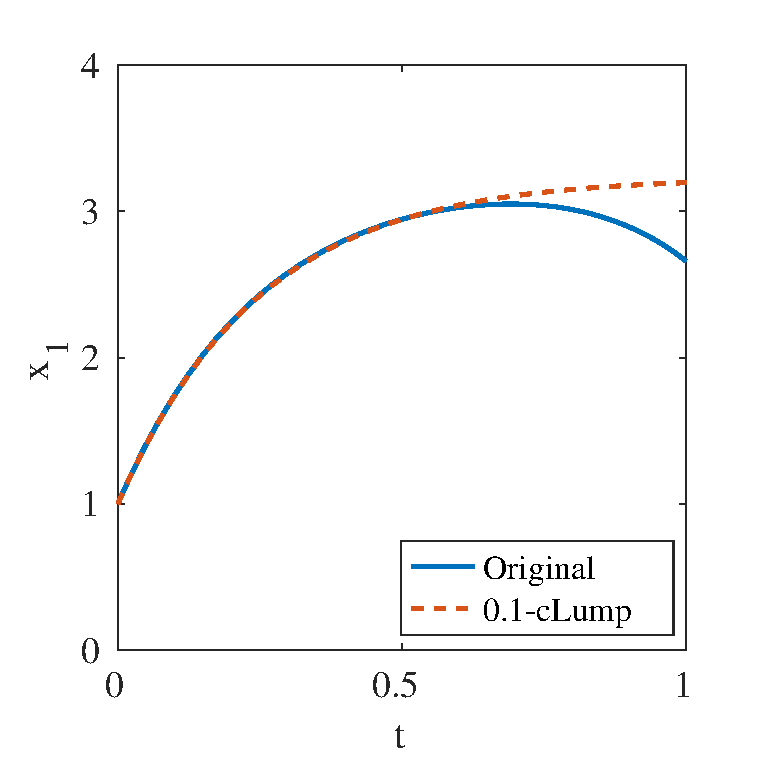
\includegraphics[width=0.35\textwidth]{img/examplecalc.pdf}
    \caption{\comalex{this is a placeholder}
        Time evolution of the $C_3$ concentration using approximate constrained lumping.}
    \label{fig:results}
\end{wrapfigure}


%We begin by getting a model from OdeBase:\\
%\mintinline{python}{)}\\
%To validate the model, we can check its validity via \texttt{model.[attribute]}, where \texttt{attribute} can be the \texttt{name}, \texttt{species}, \texttt{parameters} and \texttt{equations} among others.
%Suppose, we want to study the evolution of the observable $C_3$, this corresponds to the variable $x7$ in the model.
%To construct an exact lumping that perserves the evolution of $x7$ it suffices to use the following line. \\
%\mintinline{python}{exact_lumping = model.lumping([obs_poly])}\\
%\ToolName warns us that the exact lumping found is not a reduction as it has the same size as the original one.

%We can use \ToolName to obtain the next reduction, using the following command \\
%\mintinline{python}{app_lumping = model.app_lumping([obs_poly])}\\
%This command outputs the numerical lumping closest to the exact one.
%Different approximate lumpings can be obtained by providing a value to the \texttt{lumpingTol} keyword argument.
%Similarly, we can explore the attributes of the lumped system.
%For example, we have that \\
%\mintinline{python}{app_lumping.size}\\
%Outputs a reduction of size $12$.
%This is not a significant reduction.
%To ensure we get a small enough reduction we can use the following command \\
%\mintinline{python}{app_lumping = model.app_lumping([obs_poly], max_size=10)}\\
%which will output a reduction with a maximum size of $10$.
%In this case the computed reduction has a size of $7$.

%To see the performance of the approximate lumping we simulate both the original system from 0 to $5000~$seconds using the following lines \\
%\mintinline{python}{exact_sim = model.simulate(0, 5000)}\\
%A similar line outputs the results for the approximate lumped model.
%The simulations can then be merged using \\
%\mintinline{python}{comp_results = merge_simulations(exact_sim, app_sim)}\\
%The merged simulation can be immediately plotted by \\
%\mintinline{python}{create_figure(comp_results, title=['Original', 'Approximate'])}\\
%The resulting plot is show as follows






